\documentclass[UTF8]{ctexart}
\usepackage{graphicx} % 插入图片
\usepackage{amsmath}  % 数学公式
\usepackage{siunitx}  % 单位格式
\usepackage{caption}  % 图表标题
\usepackage{geometry} % 页面布局
\usepackage{float}    % 控制浮动体位置
\geometry{margin=1in}

\title{电饭煲的工作原理与技术解析}
\author{作者:薛中州}
\date{\today}

\begin{document}%导言之后的正文
\maketitle
\listoftables % 显示所有表格标签
\begin{abstract}%摘要的序言
\pagestyle{plain}%为了使章节的页脚明确正确
本文简要介绍了电饭煲的核心结构、加热原理及控制逻辑,结合热力学与电路基础知识,分析其如何实现米饭的自动化烹饪。
\end{abstract}

\section{电饭煲的基本结构}
电饭煲主要由以下部件组成(见图\ref{fig:rice_cooker_structure}):%pdflatex "电饭煲的原理.tex"; pdflatex "电饭煲的原理.tex",连续两次执行才能成功显示图1或图2
\begin{itemize}%无序排列
    \item \textbf{内胆}:通常为铝合金或不锈钢材质,表面附有\textbf{不粘涂层}。
    \item \textbf{加热盘}:底部电阻式加热元件,功率通常为 \SI{500}{\watt} 至 \SI{1200}{\watt}。
    \item \textbf{温度传感器}:热敏电阻或磁钢温控器,监测内胆温度。
    \item \textbf{控制电路}:包括微处理器或机械定时器,控制加热阶段切换。
\end{itemize}

\begin{figure}[ht]
    \centering
    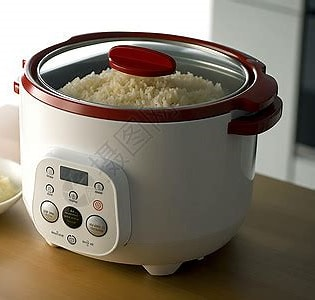
\includegraphics[width=0.6\textwidth]{images/rice_cooker_diagram.png} % 替换为实际图片路径
    \caption{电饭煲结构示意图}
    \label{fig:rice_cooker_structure}
\end{figure}

\section{工作原理}
\subsection{加热阶段}
电饭煲通过\textbf{电阻加热}将电能转化为热能,公式如下:
\begin{equation}
    P = \frac{V^2}{R}
\end{equation}
其中 \( P \) 为功率(\si{\watt}),\( V \) 为电压(\si{\volt}),\( R \) 为加热盘电阻(\si{\ohm})。

\subsection{温度控制逻辑}
现代电饭煲采用多阶段加热:
\begin{enumerate}
    \item \textbf{预热阶段}:加热至 \SI{60}{\celsius},激活淀粉酶促进吸水。
    \item \textbf{沸腾阶段}:升温至 \SI{100}{\celsius},维持沸腾状态。
    \item \textbf{焖饭阶段}:温度降至 \SI{90}{\celsius} 以下,利用余热完成淀粉糊化。
\end{enumerate}

机械式电饭煲通过\textbf{磁钢温控器}(居里点约 \SI{103}{\celsius})自动断电,而智能电饭煲使用微处理器实时调节功率(见图\ref{fig:control_logic})。

\begin{figure}[ht]
    \centering
    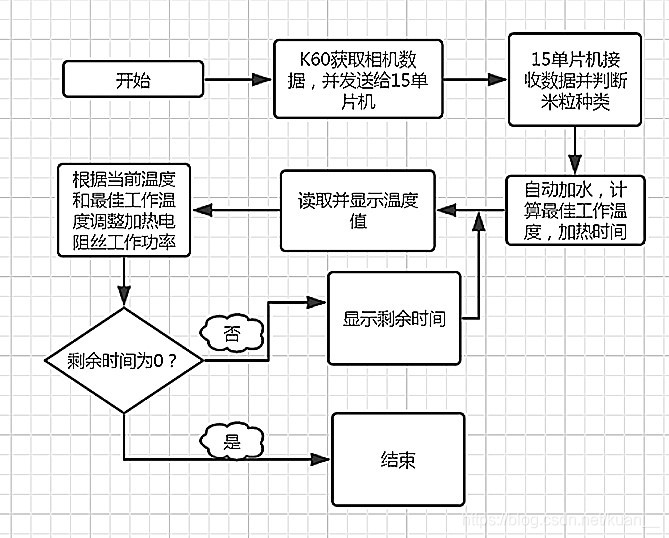
\includegraphics[width=0.8\textwidth]{images/control_logic.png} % 替换为实际流程图
    \caption{智能电饭煲控制逻辑流程图}
    \label{fig:control_logic}
\end{figure}

\section{关键技术参数}
典型电饭煲的技术规格如表\ref{tab:specs}所示:
\begin{table}[ht]%浮动体环境,允许表格在文档中自动浮动到合适位置(如页面顶部、底部)。
    \centering
    \begin{tabular}{|l|c|}%定义表格的内容和结构
        \hline
        \textbf{参数} & \textbf{数值} \\ \hline
        额定电压 & \SI{220}{\volt} \\ \hline
        功率范围 & \SI{500}{\watt} -- \SI{1200}{\watt} \\ \hline
        容量 & \SI{3}{\liter} -- \SI{5}{\liter} \\ \hline
        最高温度 & \SI{120}{\celsius} \\
         \hline
    \end{tabular}
    \caption{电饭煲典型技术参数}
    \label{tab:specs}
\end{table}

\section{安全设计}
电饭煲需满足以下安全要求:
\begin{itemize}
    \item 双重绝缘设计,防止漏电。
    \item 干烧保护:温度超过 \SI{150}{\celsius} 时自动切断电源。
    \item 蒸汽阀设计:避免内部压力过高。
\end{itemize}

\section{结论}
电饭煲通过精确的\textbf{温度-时间控制}实现米饭的完美烹饪,其核心技术包括高效加热、智能温控及安全保护机制。未来发展方向可能涉及物联网控制(如手机APP远程操作)和更精细的烹饪算法。

\end{document}